\chapter{How Sound Travels}\label{ch:g4:how-sound-travels}

The flash of lightning --- then one, two, three seconds of silence
--- and only now the growl of thunder. Yet flash and growl were
born together in the same cloud! \omterm{def:g3:sound-around-us:sound}{Sound}, we learned, is a trembling
that travels. This chapter follows it on the road: what it travels
through, how fast it runs, and what happens when it hits a wall.

\section{Sound needs a carrier}

\begin{proposition}[No carrier, no sound]\label{prop:g4:how-sound-travels:carrier}
\omterm{def:g3:sound-around-us:sound}{Sound} travels only \emph{through} things: through \omterm{def:g2:air-around-us:air}{air}, through
water, through wood, brick and steel. Where there is nothing at all
--- no \omterm{def:g2:air-around-us:air}{air}, no stuff of any kind --- \omterm{def:g3:sound-around-us:sound}{sound} cannot travel: the
trembling has nothing to tremble.
\end{proposition}

\begin{example}[The bell in the jar]\label{ex:g4:how-sound-travels:jar}
A famous experiment, three centuries old: an electric bell rings
inside a glass jar --- clearly heard. A pump then sucks the \omterm{def:g2:air-around-us:air}{air} out
of the sealed jar while the bell's hammer keeps visibly beating.
The ringing fades\dots\ and dies. Let the \omterm{def:g2:air-around-us:air}{air} rush back in: the
ringing returns. The bell never stopped --- its \emph{carrier} was
taken away and returned. And now you can settle an old question:
the silent \omterm{def:g2:moon-in-the-sky:moon}{Moon}, where a shout dies unheard, is silent because it
has no \omterm{def:g2:air-around-us:air}{air} at all.
\end{example}

\begin{omfigure}
\begin{tikzpicture}[scale=0.85]
  \draw[thick] (0.7,0) -- (0.7,3.0) .. controls (0.7,3.5) and
    (3.3,3.5) .. (3.3,3.0) -- (3.3,0);
  \draw[thick] (0.2,0) -- (3.8,0);
  % the bell: hanger, dome with a flared skirt, mouth, clapper
  \draw[thick] (2.0,2.9) -- (2.0,2.45);
  \draw[thick, fill=yellow!65!orange]
    (1.42,1.52)
    .. controls (1.5,1.6) and (1.58,1.7) .. (1.6,1.85)
    .. controls (1.62,2.1) and (1.65,2.45) .. (2.0,2.45)
    .. controls (2.35,2.45) and (2.38,2.1) .. (2.4,1.85)
    .. controls (2.42,1.7) and (2.5,1.6) .. (2.58,1.52)
    -- cycle;
  \draw[thick] (1.42,1.52) .. controls (2.0,1.43) .. (2.58,1.52);
  \fill (2.0,1.38) circle (0.07);
  \draw[omDef, dotted, thick] (1.15,1.9) arc (150:210:0.5);
  \draw[omDef, dotted, thick] (2.85,2.15) arc (30:-30:0.5);
  \node[right, font=\small] at (4.3,2.6) {sealed glass jar};
  \node[right, font=\small] at (4.3,1.8) {bell, still beating};
  \node[right, font=\small] at (4.3,1.0)
    {air pumped out: the ringing dies};
  \draw[-Stealth, thick, omExo] (3.0,0.35) -- (4.1,0.35);
  \node[right, font=\small, omExo] at (4.15,0.35) {to the pump};
\end{tikzpicture}

{\small The bell in the jar: take away the \omterm{def:g2:air-around-us:air}{air}, and the \omterm{def:g3:sound-around-us:sound}{sound} ---
not the bell --- stops.}
\end{omfigure}

\begin{example}[Better carriers than air]\label{ex:g4:how-sound-travels:solids}
\omterm{def:g3:solids-liquids-gases:solid}{Solids} and water carry \omterm{def:g3:sound-around-us:sound}{sound} wonderfully --- often better than \omterm{def:g2:air-around-us:air}{air}.
Press your ear flat on the table and have a friend scratch its far
end \emph{very} softly: through the \omterm{def:g2:air-around-us:air}{air} you hear nothing, through
the wood the scratch is loud and crisp. Swimmers hear the pool's
underwater clanks from end to end; whales sing to each other across
whole seas. And thick walls carry the neighbor's drilling into
every room --- \omterm{def:g3:solids-liquids-gases:solid}{solids} are almost too good at this.
\end{example}

\begin{method}[The string telephone]\label{met:g4:how-sound-travels:telephone}
\begin{enumerate}
  \item Punch a small hole in the bottoms of two paper cups;
  \item thread the ends of a long string in, knotting each so it
        cannot slip out;
  \item walk apart until the string is stretched \emph{tight} and
        touches nothing on the way;
  \item one speaks softly into a cup; the other holds theirs to the
        ear.
\end{enumerate}
The whisper arrives clear across the playground: your voice makes
the cup tremble, the trembling runs along the taut string, and the
far cup replays it. Let the string sag or pinch it with two
fingers, and the telephone dies --- the road is cut.
\end{method}

\begin{omfigure}
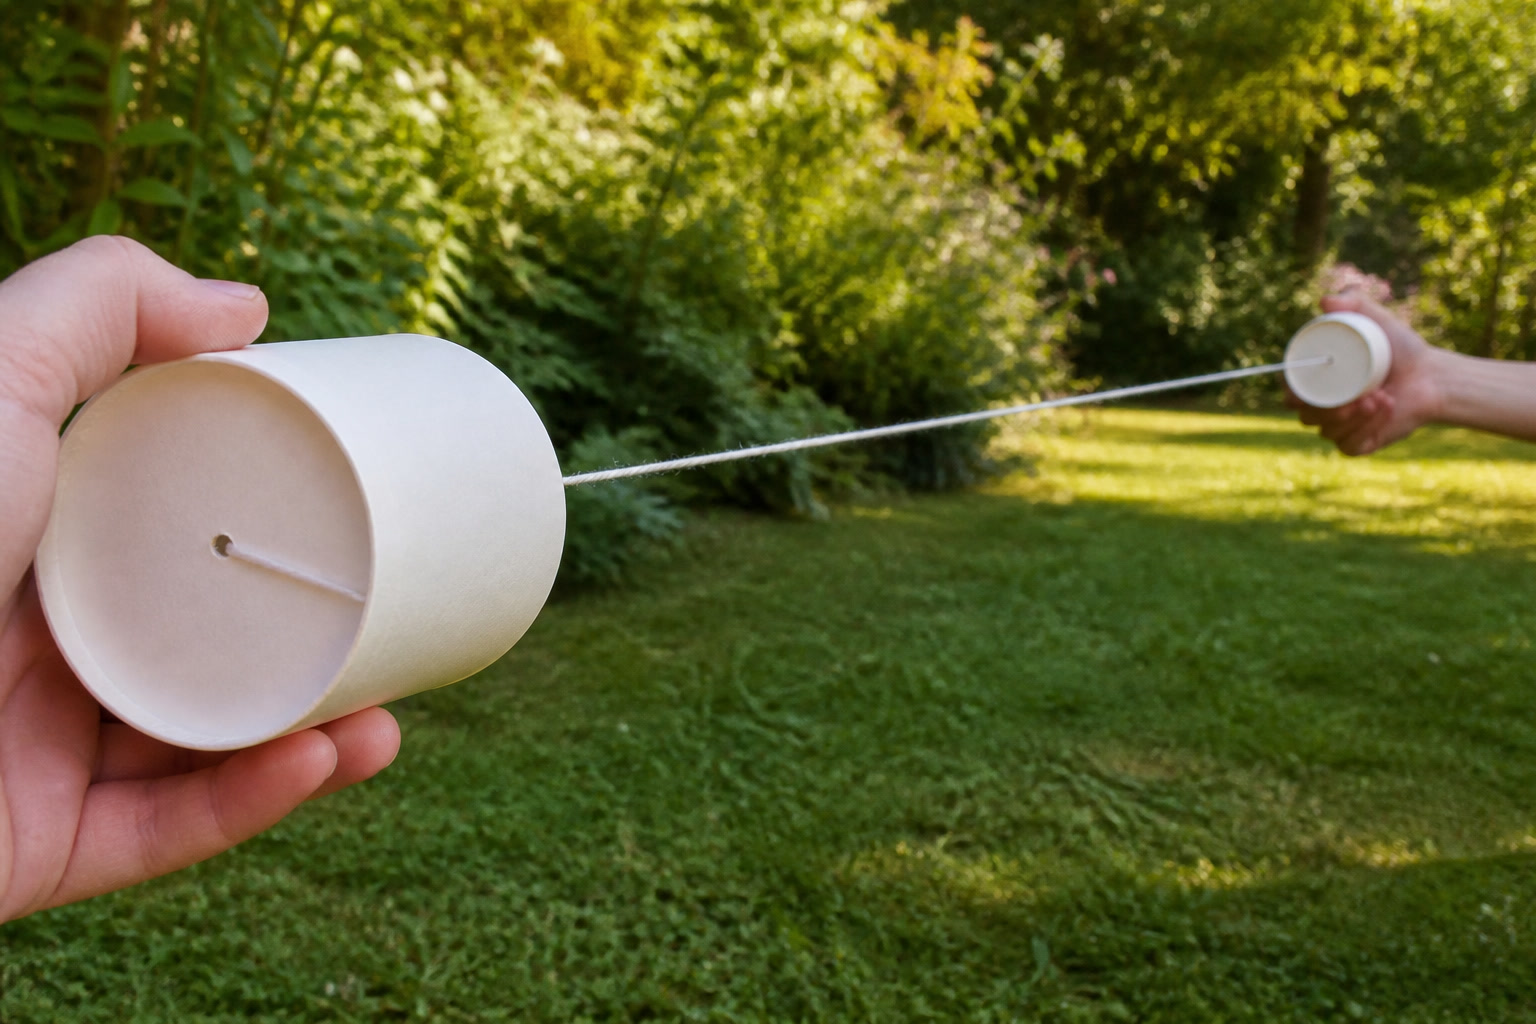
\includegraphics[width=0.58\linewidth]{images/book1/ai/g4-sound-string-telephone.jpg}

{\small The string telephone, strung and taut: a tight string carries the trembling from cup to cup far better than the \omterm{def:g2:air-around-us:air}{air} between two whisperers.}
\end{omfigure}

\section{Sound takes time}

\begin{proposition}[Fast, but not instant]\label{prop:g4:how-sound-travels:speed}
\omterm{def:g3:sound-around-us:sound}{Sound} is a runner, not a magician: in \omterm{def:g2:air-around-us:air}{air} it covers about
\qty{340}{m} in each second --- three seconds for roughly a
kilometre. \omterm{def:g1:light-and-shadows:source}{Light}, by contrast, arrives so fast that for any scene
you can watch, its trip counts as instant. That difference is the
whole story of the thunderstorm.
\end{proposition}

\begin{method}[How far is the storm?]\label{met:g4:how-sound-travels:storm}
\begin{enumerate}
  \item See the flash --- start counting seconds steadily: one
        little crocodile, two little crocodiles, \dots;
  \item stop at the first growl of thunder;
  \item divide your count by $3$: that is roughly the storm's
        distance in kilometres.
\end{enumerate}
Six seconds: about \qty{2}{km}. Counts growing shorter between
strikes mean the storm is coming closer --- time to head indoors.
\end{method}

\begin{omfigure}
\begin{tikzpicture}[scale=0.85]
  \draw[thick] (0,0) -- (11,0);
  \draw[very thick, omThm] (1.3,3.4) -- (0.9,2.5) -- (1.25,2.5)
    -- (0.8,1.5) -- (1.15,1.5) -- (0.7,0.4);
  \fill[omExo, opacity=0.3] (0.3,3.4) ellipse (1.5 and 0.45);
  % the listener, counting the silent seconds
  \fill (9.6,1.32) circle (0.18);
  \draw[thick] (9.6,1.14) -- (9.6,0.55);
  \draw[thick] (9.6,1.02) -- (9.33,0.75);
  \draw[thick] (9.6,1.02) -- (9.87,0.75);
  \draw[thick] (9.6,0.55) -- (9.4,0);
  \draw[thick] (9.6,0.55) -- (9.8,0);
  \foreach \r in {0.7, 1.4, 2.1} {
    \draw[omDef, thick] (1.0,0.4) ++(\r,0) arc (0:40:\r);
    \draw[omDef, thick] (1.0,0.4) ++(\r,0) arc (0:-12:\r);
  }
  \node[font=\small, align=center] at (9.15,2.35)
    {``\dots{}five, six''\\--- about \qty{2}{km}};
  \node[right, font=\small, omDef] at (3.6,0.75)
    {the growl, running at \qty{340}{m} each second};
\end{tikzpicture}

{\small Flash now, thunder later: \omterm{def:g1:light-and-shadows:source}{light} arrives at once, \omterm{def:g3:sound-around-us:sound}{sound} jogs
across at \qty{340}{m} per second. The silent seconds \omterm{def:g2:measuring-length:measure}{measure} the
distance.}
\end{omfigure}

\begin{example}[Echoes]\label{ex:g4:how-sound-travels:echo}
Shout toward a big cliff or a lone building far across a field:
``HELLO!'' --- a moment of silence --- ``Hello!'' answers your own
voice. \omterm{def:g3:sound-around-us:sound}{Sound} bounces off large hard walls, and a bounced \omterm{def:g3:sound-around-us:sound}{sound} that
returns to you late enough to hear separately is an
\emph{echo}\index{echo}. The farther the wall, the longer your
voice's round trip, the later the \omterm{ex:g4:how-sound-travels:echo}{echo}. In a small room the bounce
comes back too quickly to hear apart --- it only makes your voice
\omterm{def:g3:sound-around-us:sound}{sound} fuller.
\end{example}

\begin{remark}[Sonar: the echo put to work]\label{rem:g4:how-sound-travels:sonar}
Ships \omterm{def:g2:measuring-length:measure}{measure} the sea's depth by shouting downward --- a click into
the water --- and timing the \omterm{ex:g4:how-sound-travels:echo}{echo} from the bottom. Deep water,
late \omterm{ex:g4:how-sound-travels:echo}{echo}; shallow water, quick \omterm{ex:g4:how-sound-travels:echo}{echo}. Dolphins and bats were born
knowing the trick: they click and listen, reading the \omterm{ex:g4:how-sound-travels:echo}{echoes} to
hunt in dark water and pitch-black caves. Counting thunder-seconds,
you have already used their method: time the \omterm{def:g3:sound-around-us:sound}{sound}, know the
distance.
\end{remark}

\section{Exercises}

\begin{exercise}[$\star$]\label{exo:g4:how-sound-travels:1}
Name three carriers of \omterm{def:g3:sound-around-us:sound}{sound} from this chapter, and one place where
\omterm{def:g3:sound-around-us:sound}{sound} cannot travel at all.
\end{exercise}

\begin{exercise}[$\star$]\label{exo:g4:how-sound-travels:2}
In the jar experiment, the bell's hammer keeps beating while the
ringing dies. What exactly was taken away, and what does that
prove?
\end{exercise}

\begin{exercise}[$\star$]\label{exo:g4:how-sound-travels:3}
Why is the \omterm{def:g2:moon-in-the-sky:moon}{Moon} a silent world? Answer with the proposition of the
chapter.
\end{exercise}

\begin{exercise}[$\star$]\label{exo:g4:how-sound-travels:4}
In the string telephone, what carries the whisper? Give both rules
for keeping the telephone working.
\end{exercise}

\begin{exercise}[$\star$]\label{exo:g4:how-sound-travels:5}
About how far does \omterm{def:g3:sound-around-us:sound}{sound} travel through \omterm{def:g2:air-around-us:air}{air} in one second? In three
seconds?
\end{exercise}

\begin{exercise}[$\star$]\label{exo:g4:how-sound-travels:6}
You count nine seconds between flash and thunder. How far is the
storm? Your friend counts only three seconds at the next strike ---
what has changed, and what should you both do?
\end{exercise}

\begin{exercise}[$\star$]\label{exo:g4:how-sound-travels:7}
Why does pressing an ear to the table let you hear a scratch that
the \omterm{def:g2:air-around-us:air}{air} never delivered?
\end{exercise}

\begin{exercise}[$\star$]\label{exo:g4:how-sound-travels:8}
What is an \omterm{ex:g4:how-sound-travels:echo}{echo}? Why does a bigger, farther cliff answer later than
a near one?
\end{exercise}

\begin{exercise}[$\star$]\label{exo:g4:how-sound-travels:9}
How does a ship's sonar tell deep water from shallow? Which two
animals play the same game, and where?
\end{exercise}

\begin{exercise}[$\star\star$]\label{exo:g4:how-sound-travels:10}
Old westerns show scouts pressing an ear to the steel rail to catch
a still-distant train. Why does the rail betray the train long
before the \omterm{def:g2:air-around-us:air}{air} does? Give both advantages the rail offers to the
\omterm{def:g3:sound-around-us:sound}{sound}. (One is about carrying well; for the other, remember that
the rail runs straight to the train while \omterm{def:g3:sound-around-us:sound}{sound} in \omterm{def:g2:air-around-us:air}{air} spreads out
in every direction like pond rings, thinning as it goes.)
\end{exercise}

\begin{exercise}[$\star\star$]\label{exo:g4:how-sound-travels:11}
Standing in a big empty courtyard, you clap once and hear the slap
of your own clap return from the far wall after one full second.
\omterm{def:g3:sound-around-us:sound}{Sound} ran to the wall and back in that second. How far away is the
wall --- careful, think about the round trip!
\end{exercise}
